
% ============================================================================
% CONCEPTION STRUCTURELLE - MODÈLE DE DONNÉES
% MONDJO NZUKAM VANELLE SANDRA - Matricule: 25I2283
% ============================================================================

\chapter{Conception Structurelle des Données}
\textit{La conception structurelle des données constitue le socle du cahier de texte digital. Elle définit la manière dont l'information relative aux utilisateurs, aux classes, aux matières, aux séances, aux devoirs et aux absences est organisée, stockée et mise en relation au sein du système de base de données.}

\section{Entités Identifiées}

\textit{L'analyse du domaine fonctionnel du cahier de texte digital a permis d'identifier neuf entités principales. Chaque entité représente un objet du monde réel dont les attributs sont persistés en base de données.}

% Consultez le fichier MONDJO/task.tex pour les ressources complètes
% Décrire chaque entité avec ses attributs et contraintes

\subsection{Entité UTILISATEUR}

\textit{Représente Tout être utilisant le système (enseignant, étudiant, parent, admin)}

\begin{center}
    
\begin{tabular}{|l|c|r|a|} 
  \hline 
  \textbf{Attributs} & \textbf{Type} & \textbf{Contrainte} & \textbf{Description}\\
  \hline
  id\_utilisateur & INT & PK & identifiant unique \\
  \hline
  nom & VARCHAR 100 & NOT NULL & Nom complet \\
  \hline
  email & VARCHAR 100 & UNIQUE & Email unique \\
  \hline
  mot\_de\_passe\_hash & VARCHAR 255 & NOT NULL & Hash du mot de passe (jamais en clair) \\
  \hline
  numéro\_téléphone & VARCHAR 20 & UNIQUE & Pour contact \\
  \hline
  date\_création & TIMESTAMP & DEFAULT NOW & date et heure de création \\
  \hline
  type & ENUM & NOT NULL & enseignant, étudiant, parent, admin \\
  \hline
  derniere\_connexion & TIMESTAMP & NOT NULL & Dernière activité \\
  \hline
  actif & BOOLEAN & default=true & Compte désactivable \\
  \hline
\end{tabular}
\end{center}

\subsection{Entité CLASSE}

\textit{Représente une classe scolaire (groupe d'étudiants)}
\begin{center}
    \begin{tabular}{|l|c|r|p{8cm}|}
  \hline
   \textbf{Attributs} & \textbf{Type} & \textbf{Contrainte} & \textbf{Description}\\
  \hline
  id\_classe & INT & PK & identifiant unique \\
  \hline
  nom & VARCHAR 50 & NOT NULL & libellé de la classe Ex: "Terminale A1" \\
  \hline
  niveau & VARCHAR 20 & NOT NULL & niveau scolaire Ex: "Terminale", "Seconde", "Première" \\
  \hline
  effectif & INT & NOT NULL & Nombre d'étudiants \\
  \hline
  id\_professeur\_principal & INT &  FK & reference vers Enseignant principal \\
  \hline
  annee\_scolaire & VARCHAR 20 & NOT NULL & Année scolaire Ex: "2024/2025" \\
  \hline
\end{tabular}
\end{center}

\subsection{Entité MATIERE}

\textit{Représente une matière scolaire}
\begin{center}
    \begin{tabular}{|l|c|r|p{8cm}|}
  \hline
  \textbf{Attributs} & \textbf{Type} & \textbf{Contrainte} & \textbf{Description}\\
  \hline
  id\_matière & INT & PK & identifiant unique \\
  \hline
  nom & VARCHAR 100 & NOT NULL & nom de la matière Ex: "Mathématiques", "Français" \\
  \hline
  code & VARCHAR 20 & UNIQUE &  Code académique\\
  \hline
  description & TEXT & NULLABLE & Description détaillée \\
  \hline
  id\_classe & INT & FK & Classe concernée \\
  \hline
  id\_enseignant & INT & FK & Enseignant responsable \\
  \hline
  horaire\_hebdo & INT & NOT NULL & Heures par semaine \\
  \hline
\end{tabular}
\end{center}

\subsection{Entité SÉANCE}

\textit{Représente une séance de cours enregistrée}
\begin{center}
    \begin{tabular}{|l|c|r|a|}
  \hline
  \textbf{Attributs} & \textbf{Type} & \textbf{Contrainte} & \textbf{Description} \\
  \hline
  id\_séance & INT & PK & identifiant unique \\
  \hline
  id\_matière & INT & FK &  Matière enseignée \\
  \hline
  date & DATE & NOT NULL &  Date de la séance \\ 
  \hline
  heure\_début & TIME & NOT NULL & Heure de début \\
  \hline
  heure\_fin & TIME & NOT NULL &  Heure de fin \\
  \hline
  contenu & TEXT & NULLABLE & Contenu du cours (ce qui a été abordé) \\
  \hline
  matériel & TEXT & NOT NULL &  Matériel utilisé \\
  \hline
  id\_enseignant & INT & FK &  Qui l'a saisie \\
  \hline
  validée & BOOLEAN & default=false &  Approuvée par admin ? \\
  \hline
  id\_admin\_validateur & INT & FK & Qui a validé \\
  \hline
  remarques\_admin & TEXT & NOT NULL & Notes de validation \\
  \hline
  date\_création & TIMESTAMP & NOT NULL & Quand créée \\ 
  \hline
  date\_modification & TIMESTAMP & NOT NULL & Dernière modif \\
  \hline
  date\_validation & TIMESTAMP & NOT NULL & Quand validée \\ 
  \hline
\end{tabular}
\end{center}

 \item Règle métier :
 \begin{itemize}
      \item Une séance non-validée peut être modifiée par l'enseignant
      \item Une séance validée devient read-only
    \end{itemize}
\end{itemize}  

\subsection{Entité DEVOIR}

\textit{Représente un devoir assigné aux étudiants}
\begin{center}
   \begin{tabular}{|l|c|r|a|}
  \hline
  \textbf{Attributs} & \textbf{Type} & \textbf{Contrainte} & \textbf{Description} \\
  \hline
  id\_devoir & INT & PK & identifiant unique \\
  \hline
  id\_séance & INT & FK &  Séance d'assignation \\
  \hline
  description & TEXT & NULLABLE & Description du devoir \\
  \hline
  date\_remise & DATE & NOT NULL & Date limite \\
  \hline
  type & ENUM & NOT NULL & type: exercice, projet, lecture, dissertation, autre) \\
  \hline
  obligatoire & BOOLEAN & default=true &  Devoir obligatoire ? \\
  \hline
  barème & INT & NOT NULL & Points totaux \\
  \hline
  fichier\_joint & VARCHAR 255 & NOT NULL & Nom du fichier si fourni \\
  \hline
  date\_création & TIMESTAMP & CHECK \\
  \hline
\end{tabular} 
\end{center}


\subsection{Entité ABSENCE}

\textit{Représente l'absence d'un étudiant à une séance}
\begin{center}
    \begin{tabular}{|l|c|r|a|}
  \hline
  \textbf{Attributs} & \textbf{Type} & \textbf{Contrainte} & \textbf{Description} \\
  \hline
  id\_absence & INT & PK & identifiant unique \\
  \hline
  id\_étudiant & INT & FK & Étudiant absent\\
  \hline
  id\_séance & INT & FK & Séance manquée\\
  \hline
  date & DATE & DEFAULT NOW & Date de l'absence\\
  \hline
  justifiée & BOOLEAN & default=false &  Absence justifiée ? \\
\hline
raison & TEXT & NOT NULL & Raison (si justifiée)\\
\hline
date\_enregistrement & TIMESTAMP & NOT NULL &\\
\hline
id\_enregistre\_par & INT & FK & Qui a enregistré \\
\hline
  \end{tabular}
\end{center}


\underline{\textbf{Entité RELATION PARENT-ENFANT}}
\begin{itemize}
  \item Représente : Lien parent-étudiant (un parent peut avoir plusieurs enfants)
  \item Attributs :
    \begin{itemize}
      \item id (INT, PK)
      \item id\_parent (INT, FK vers UTILISATEUR) - Parent (type=parent)
      \item id\_etudiant (INT, FK vers UTILISATEUR) - Enfant (type=etudiant)
      \item lien (ENUM: père, mère, tuteur, autre) - Relation
      \item date\_creation (TIMESTAMP)
    \end{itemize}
  \item Contraintes :
    \begin{itemize}
      \item PK: id
      \item FK: id\_parent → UTILISATEUR.id (type=parent)
      \item FK: id\_etudiant → UTILISATEUR.id (type=etudiant)
      \item UNIQUE: (id\_parent, id\_etudiant)
      \item NOT NULL: id\_parent, id\_etudiant, lien
    \end{itemize}
\end{itemize}

\underline{\textbf{Entité RELATION ETUDIANT-CLASSE}}
\begin{itemize}
  \item Représente : Inscription d'un étudiant à une classe
  \item Attributs :
    \begin{itemize}
      \item id (INT, PK)
      \item id\_etudiant (INT, FK vers UTILISATEUR) - Étudiant
      \item id\_classe (INT, FK vers CLASSE) - Classe
      \item date\_inscription (DATE) - Quand inscrit
      \item date\_desinscription (DATE, optionnel) - Si retiré plus tard
    \end{itemize}
  \item Contraintes :
    \begin{itemize}
      \item PK: id
      \item FK: id\_etudiant → UTILISATEUR.id (type=etudiant)
      \item FK: id\_classe → CLASSE.id
      \item UNIQUE: (id\_etudiant, id\_classe, date\_inscription)
    \end{itemize}
\end{itemize}

\underline{\textbf{Entité AUDIT\_LOG}}
\begin{itemize}
  \item Représente : Trace de chaque action dans le système (immuable)
  \item Attributs :
    \begin{itemize}
      \item id (INT, PK)
      \item id\_utilisateur (INT, FK vers UTILISATEUR) - Qui a fait l'action
      \item action (VARCHAR 50) - CREATE, UPDATE, DELETE, LOGIN, etc.
      \item table\_name (VARCHAR 50) - Quelle table affectée
      \item record\_id (INT) - ID du record modifié
      \item ancienne\_valeur (JSON, optionnel) - État avant (pour UPDATE)
      \item nouvelle\_valeur (JSON, optionnel) - État après (pour UPDATE)
      \item date\_action (TIMESTAMP) - Quand l'action
      \item ip\_address (VARCHAR 20) - Adresse IP source
      \item user\_agent (VARCHAR 255, optionnel) - Navigateur
    \end{itemize}
  \item Contraintes :
    \begin{itemize}
      \item PK: id
      \item FK: id\_utilisateur → UTILISATEUR.id
      \item NOT NULL: id\_utilisateur, action, table\_name, date\_action
      \item Immuable : Pas de UPDATE/DELETE, seule insertion
    \end{itemize}
\end{itemize}

\section{Relations et Cardinalités}

  \begin{center}
      
\begin{tabularx}{\textwidth}{|X|X|X|}
  \hline
  \textbf{Relation} & \textbf{Cardinalité} & \textbf{Explication} \\
  \hline
  
  UTILISATEUR → CLASSE (professeur principal) &
  1:N &
  Un enseignant peut être prof principal d'une classe, une classe a un prof principal \\
  \hline
  
  UTILISATEUR → MATIÈRE (enseignant) &
  1:N &
  Un enseignant enseigne plusieurs matières, une matière est enseignée par un enseignant \\
  \hline
  
  CLASSE → MATIÈRE &
  1:N &
  Une classe a plusieurs matières, une matière appartient à une classe \\
  \hline
  
  MATIÈRE → SÉANCE &
  1:N &
  Une matière a plusieurs séances, une séance est pour une matière \\
  \hline
  
  SÉANCE → DEVOIR &
  1:N &
  Une séance peut avoir plusieurs devoirs, un devoir est assigné dans une séance \\
  \hline
  
  SÉANCE → ABSENCE &
  1:N &
  Une séance peut avoir plusieurs absences, une absence est pour une séance \\
  \hline
  
  UTILISATEUR → ABSENCE (étudiant) &
  1:N &
  Un étudiant a plusieurs absences, une absence concerne un étudiant \\
  \hline
  
  UTILISATEUR → PARENT-ENFANT &
  N:N &
  Un parent a plusieurs enfants, un enfant peut avoir plusieurs parents/tuteurs \\
  \hline
  
  UTILISATEUR → ÉTUDIANT-CLASSE &
  N:N &
  Un étudiant peut être dans plusieurs classes (ex: changement), une classe a plusieurs étudiants \\
  \hline
\end{tabularx}
\end{center}

\newpage
\section{Diagramme Entité-Relation (E-R)}
\begin{figure}[h]
    \centering
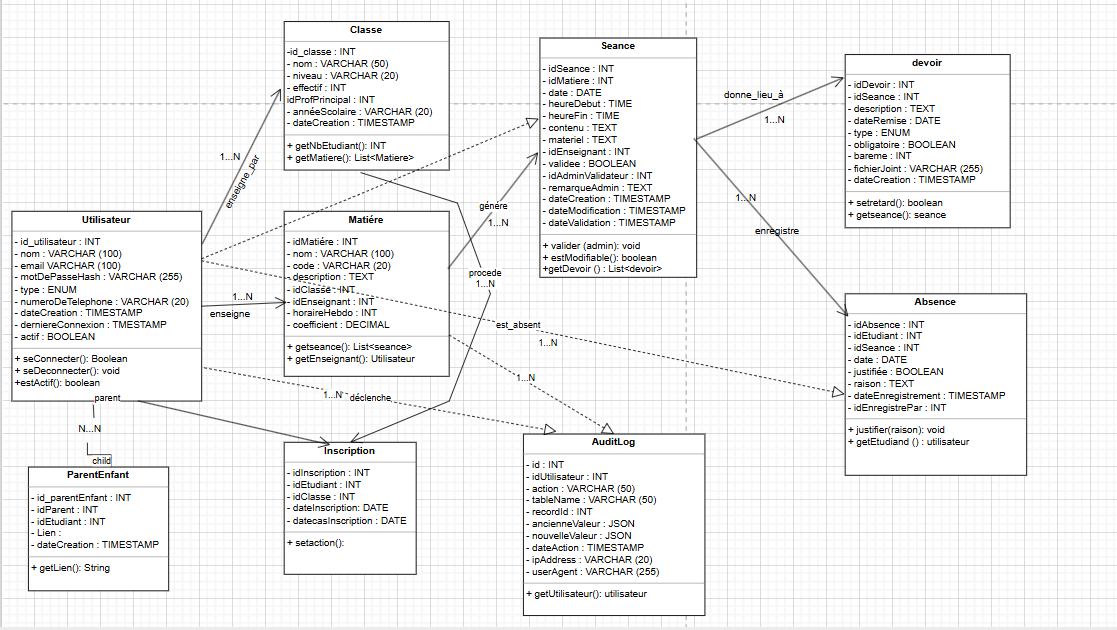
\includegraphics[width=1\linewidth]{ressources/diagram.png}
    \caption{Diagramme de classe du systéme}
    \label{fig:placeholder}
\end{figure}
    


\section{Schéma Relationnel}
\begin{center}
    
\begin{itemize}
    \item UTILISATEUR : (id, nom, email [UQ], mot_de_passe_hash, type, numéro_telephone*, date_création, derniere_connexion*, actif)
\item CLASSE : (id, nom, niveau, effectif*, #id_professeur_principal, année_scolaire,
date_création)
\item MATIERE : (id, nom, code [UQ], description*, #id_classe, #id_enseignant,
horaire_hebdo*, coefficient)
\item SEANCE : (id, #id_matiere, date, heure_debut, heure_fin, contenu, materiel*,
#id_enseignant, validee, #id_admin_validateur*, remarques_admin*,
date_creation, date_modification*, date_validation*)
\item DEVOIR : (id, #id_seance, description, date_remise, type, obligatoire, bareme*,
fichier_joint*, date_creation)
\item ABSENCE : (id, #id_etudiant, #id_seance, date, justifiee, raison*,
date_enregistrement, #id_enregistre_par [UQ(id_etudiant, id_seance)])
\item PARENT_ENFANT : (id, #id_parent, #id_etudiant, lien, date_creation [UQ(id_parent, id_etudiant)])
\item INSCRIPTION : (id, #id_etudiant, #id_classe, date_inscription, date_desinscription [UQ(id_etudiant, id_classe, date_inscription)])
\item AUDIT_LOG : (id, #id_utilisateur, action, table_name, record_id*, ancienne_valeur*, nouvelle_valeur*, date_action, ip_address, user_agent*)

\end{itemize}
 \end{center}
Convention : \underline{attribut} = PK \quad \texttt{\#attribut} = FK
\quad \texttt{attribut*} = nullable \quad \texttt{[UQ]} = UNIQUE
 
  



\section{Normalisation et Intégrité}

\textit{ Normalization (3NF - Third Normal Form)}

La conception respecte la 3e forme normale :
\begin{itemize}
  \item Pas de dépendances transitives (chaque attribut dépend uniquement de la clé primaire)
  \item Pas de colonnes redondantes (ex: pas de « nom\_enseignant » dans SÉANCE, on a id\_enseignant)
  \item Atomicité : Chaque colonne contient une valeur indivisible
\end{itemize}

\section{Indexes et Performance}

\textbf{4. Indexes pour Performance}

\underline{\textbf{Indexes à créer}}
\begin{itemize}
  \item Index sur UTILISATEUR.email (recherche fréquente pour login)
  \item Index sur SÉANCE.date (filtrage par date)
  \item Index sur SÉANCE.validée (listing des séances en attente)
  \item Index composé sur SÉANCE.(id\_matière, date) (requête commune)
  \item Index sur ABSENCE.(id\_étudiant, date) (requête présence/absence)
  \item Index sur AUDIT\_LOG.date\_action (logs récents)
\end{itemize}

\vfill